% Options for packages loaded elsewhere
\PassOptionsToPackage{unicode}{hyperref}
\PassOptionsToPackage{hyphens}{url}
%
\documentclass[
]{book}
\usepackage{amsmath,amssymb}
\usepackage{iftex}
\ifPDFTeX
  \usepackage[T1]{fontenc}
  \usepackage[utf8]{inputenc}
  \usepackage{textcomp} % provide euro and other symbols
\else % if luatex or xetex
  \usepackage{unicode-math} % this also loads fontspec
  \defaultfontfeatures{Scale=MatchLowercase}
  \defaultfontfeatures[\rmfamily]{Ligatures=TeX,Scale=1}
\fi
\usepackage{lmodern}
\ifPDFTeX\else
  % xetex/luatex font selection
\fi
% Use upquote if available, for straight quotes in verbatim environments
\IfFileExists{upquote.sty}{\usepackage{upquote}}{}
\IfFileExists{microtype.sty}{% use microtype if available
  \usepackage[]{microtype}
  \UseMicrotypeSet[protrusion]{basicmath} % disable protrusion for tt fonts
}{}
\makeatletter
\@ifundefined{KOMAClassName}{% if non-KOMA class
  \IfFileExists{parskip.sty}{%
    \usepackage{parskip}
  }{% else
    \setlength{\parindent}{0pt}
    \setlength{\parskip}{6pt plus 2pt minus 1pt}}
}{% if KOMA class
  \KOMAoptions{parskip=half}}
\makeatother
\usepackage{xcolor}
\usepackage{graphicx}
\makeatletter
\newsavebox\pandoc@box
\newcommand*\pandocbounded[1]{% scales image to fit in text height/width
  \sbox\pandoc@box{#1}%
  \Gscale@div\@tempa{\textheight}{\dimexpr\ht\pandoc@box+\dp\pandoc@box\relax}%
  \Gscale@div\@tempb{\linewidth}{\wd\pandoc@box}%
  \ifdim\@tempb\p@<\@tempa\p@\let\@tempa\@tempb\fi% select the smaller of both
  \ifdim\@tempa\p@<\p@\scalebox{\@tempa}{\usebox\pandoc@box}%
  \else\usebox{\pandoc@box}%
  \fi%
}
% Set default figure placement to htbp
\def\fps@figure{htbp}
\makeatother
\setlength{\emergencystretch}{3em} % prevent overfull lines
\providecommand{\tightlist}{%
  \setlength{\itemsep}{0pt}\setlength{\parskip}{0pt}}
\setcounter{secnumdepth}{5}
\ifLuaTeX
\usepackage[bidi=basic]{babel}
\else
\usepackage[bidi=default]{babel}
\fi
\babelprovide[main,import]{italian}
% get rid of language-specific shorthands (see #6817):
\let\LanguageShortHands\languageshorthands
\def\languageshorthands#1{}
          \usepackage{cancel}
          \usepackage{float}
          \usepackage{subcaption}
          \usepackage{tikz}
          \usepackage[version=4]{mhchem}
          \usepackage{circuitikz}
          \usepackage{steinmetz}
          \usepackage{derivative}
          \usepackage{tabularray}
          \usepackage{mathtools}
          \usepackage{siunitx}
          \usepackage{tcolorbox}
          \usepackage{geometry}
          \usepackage{array}
          \usepackage{caption}
          \usepackage{sectsty}
          \usepackage{hhline}
              \geometry{
                  a4paper,
                  total={170mm,257mm},
                  left=20mm,
                  top=20mm,
              }
          \tcbuselibrary{most}
          \newtcolorbox[auto counter,number within=section]{mybox}[1]{colback=red!5!white, colframe=red!75!black,
          fonttitle=\bfseries, title={#1}}
\usepackage{bookmark}
\IfFileExists{xurl.sty}{\usepackage{xurl}}{} % add URL line breaks if available
\urlstyle{same}
\hypersetup{
  pdftitle={Appunti Elettronica Digitale},
  pdfauthor={Leonardo Toccafondi},
  pdflang={it},
  pdfsubject={Elettronica},
  hidelinks,
  pdfcreator={LaTeX via pandoc}}

\title{Appunti Elettronica Digitale}
\author{Leonardo Toccafondi}
\date{2024-04-12}

\begin{document}
\frontmatter
\maketitle

{
\setcounter{tocdepth}{2}
\tableofcontents
}
\mainmatter
\chapter{Dispositivi elettronici}\label{dispositivi-elettronici}

\section{Semiconduttori}\label{semiconduttori}

I semiconduttori sono i materiali con cui sono composti i circuiti
integrati. Sono, come suggerisce il nome, materiali in cui il flusso di
corrente \emph{non è libero} (non è un conduttore), ma è
\textbf{presente} (non è un'isolante).

In particolare, conducono in particolari situazioni. Quali sono però i
materiali con queste condizioni?

\begin{itemize}
\tightlist
\item
  \emph{Elementi semiconduttori}: Silicio (\ce{Si}), Germanio (\ce{Ge})
  (Carbonio (\ce{C}), ma composto)
\item
  \emph{Elementi composti}: \ce{GaAs}, \ce{GaN} (Gallio-Arsenico/Azoto)
  In generale sono gli elementi della \(4°\) colonna della tavola
  periodica o composti a numero medio di elettroni liberi pari a 4 (dai
  3 ai 4).
\end{itemize}

\begin{mybox}{\emph{Silicio}}
Il silicio è il materiale semiconduttore sicuramente più diffuso. \newline
Un atomo presenta 4 elettroni (detti di \emph{valenza}) nello strato più esterno,
ma sua forma cristallina pura del silicio ogni atomo forma un legame covalente
\footnote{legame chimico in cui due atomi mettono in comune delle coppie di elettroni.}
con i suoi vicini "più prossimi".
Il cristallo di silicio puro ha inoltre una struttura cristallina matriciale,
che blocca il passaggio di carica. \newline
È da notare che all'aumentare della temperatura, qualche elettrone può rompere il legame
e muoversi liberamente nel cristallo.
\end{mybox}

Per dotare un materiale semiconduttore di conduttività \emph{selettiva}
è necessario \emph{``drogare''} il materiale stesso. Il drogaggio,
quindi, va a \textbf{modificare} la concentrazione di elettroni e di
\emph{lacune} \footnote{Assenza di elettroni dovuta alla
  \textbf{rottura} di un legame. È insieme all'elettrone, un portatore
  di carica nei semiconduttori.}, attraverso questo inserimento di
impurità sostituzionali (ovvero atomi di elementi diversi, i quali si
sostituiscono ad alcuni degli atomi di silicio.) \newline In pratica
andiamo ad aggiungere, in piccole dosi, nel reticolo cristallino
materiali della \(5°\) colonna (drogaggio di tipo \textbf{n}, hanno 5
elettroni di valenza, sono detti \textbf{donatori}, ad esempio il
fosforo), o elementi della \(3°\) colonna (tipo \textbf{p}, hanno 3
elettroni di valenza e sono detti \textbf{accettori}, ad esempio il
boro).\newline Tale discrepanza induce la formazione di livelli
energetici aggiuntivi all'interno della banda proibita\footnote{Intervallo
  di energia interdetto agli elettroni, distanza tra la banda di valenza
  di conduzione (nei semiconduttori distanti \(1\si{eV}\)).} o ``gap''
del semiconduttore. Nel primo caso si genera un eccesso di lacune, le
quali si comportano come particelle cariche \emph{positivamente}, mentre
nel secondo si ha un eccesso di elettroni liberi, determinando così una
variazione della conducibilità elettrica intrinseca del materiale.
\newline Non solo, sia le lacune che gli elettroni liberi sono quindi
liberi di muoversi all'interno del semiconduttore!

La qualità del semiconduttore è influenzata dal materiale usato (per
esempio Ge è meglio del \ce{Si}, ma è più raro), che è a sua volta
influenzato dal goal\footnote{(penso voglia dire ``obiettivo
  perseguito'').} (elettronica digitale usa \ce{Si}, l'elettronica di
potenza il \ce{GaN} o \ce{SiC}).

Vediamo ora degli elementi in silicio.

\subsection{Giunzione p-n}\label{giunzione-p-n}

Una giunzione pn (o p-n) si forma quando una del materiale
semiconduttore intrinseco \footnote{Puro, quindi privo di un
  quantitativo significativo di drogaggio.} drogato con un drogaggio p
(con una percentuale \(N_{A}\), n.~accettori) viene posta a contatto con
altro materiale semiconduttore drogato con un drogaggio n (con una
percentuale \(N_{D}\), n.~donatori). \newline La concentrazione di ioni
dalle seguenti ``formule'': \[
N_A = \frac{\# acceptors}{vol. unit} \text{ e } N_D=\frac{\# donors}{vol. unit}
\] dove \(N_a\) indica il numero\footnote{Oppure densità di ioni, o
  concentrazione\ldots{}} di ioni di tipo p:`positivo', mentre \(N_d\)
il numero di ioni di tipo n:`negativo'.

Collegando un blocco drogato tipo p ed uno tipo n abbiamo
(idealmente)\footnote{Nella pratica parto da un blocco puro di silicio,
  per poi iniettare a \emph{strati} il drogaggio.}

\begin{figure}[H]
\centering
\begin{tikzpicture}[scale=1.75]
    \draw[very thick](-2,0)--(2,0)--(2,1)--(-2,1)--(-2,0);
    \draw[very thick](0,0)--(0,1);
    \draw[thick](0.5,0)--(0.5,1);
    \draw[thick](-0.5,0)--(-0.5,1);
    \node at (1.25,0.5) {$N$};
    \node at (-1.25,0.5) {$P$};
     % Aggiungiamo le due righe orizzontali
    \draw[thick](-2.5,0.5)--(-2,0.5);
    \draw[thick](2,0.5)--(2.5,0.5);
    \draw[->](-0.25,0.5)--(0.25,0.5)node[above]{$V_0$};
\end{tikzpicture}
\caption{Giunzione pn}
\end{figure}

Il materiale quindi è separato in due zone \emph{nettamente distinte},
senza alterazione della struttura cristallina all'interfaccia delle due
zone. \newline

L'abbondanza di lacune in p è, come sappiamo, corrispondente ad una
carenza di elettroni, di cui n \emph{abbonda}. In altre parole questa
diversa \emph{densità} di portatori di carica genera una
\textbf{migrazione} di elettroni da N verso P, detta anche
\emph{diffusione\footnote{Fenomeno che si ritrova in natura qualora vi
  sia uno squilibrio nella distribuzione nello spazio di particelle
  simili.} (elettrica)} \(I_D\) oppure anche \emph{corrente di
diffusione}, che consiste quindi in

\begin{itemize}
\tightlist
\item
  lacune che si diffondono dalla regione (dal semiconduttore) drogata
  con p alla regione n;
\item
  elettroni che si diffondono dalla regione drogata con n alla regione
  p.
\end{itemize}

\begin{quote}
N.B.: Nella zona n i \textbf{portatori maggioritari} di carica sono le
cariche negative, mentre nella zona p sono le cariche positive
\end{quote}

Tale fenomeno carica in modo \emph{positivo} il semiconduttore drogato n
(meno elettroni), e in modo \emph{negativo} il semiconduttore drogato p
(più elettroni). \newline Le lacune che si diffondono dalla regione/zona
p alla n si ricombinano con gli elettroni liberi, \emph{scomparendo}. Di
conseguenza, il numero di elettroni liberi nella zona n
\emph{diminuisce}, quindi non saranno più neutralizzate alcune cariche
fisse positive (atomi donatori). Dal momento che questa ricombinazione
avviene in prossimità della giunzione, accanto a questa si svilupperà
una regione \textbf{svuotata} di elettroni, con cariche fisse positive
non compensate. \newline Analogamente nella zona p otterremo una zona
svuotata dalle lacune e che comprende delle cariche fisse (in questo
caso negative) non compensate. \newline Entrambe queste zone danno luogo
alla \textbf{regione di svuotamento}\footnote{Svuotata di portatori
  \textbf{mobili}} (o di carica spaziale, in inglese \emph{depletion
layer}). Inoltre lo spostamento delle cariche crea a cavallo della
giunzione un campo elettrico, con la zona n positiva rispetto alla zona
p.~La presenza del campo elettrico comporta la presenza di una
differenza di potenziale. Questa è anche detta \textbf{barriera di
potenziale}\footnote{È possibile superarla, ma deve essere fornita una
  differenza di potenziale \textbf{esterna}.}, in quanto si oppone ad
un'ulterore diffusione ai portatori di carica soggetti alla spinta della
diffusione (si oppone al movimento di elettroni nella regione p e lacune
nella regione n). Una volta che la corrente di diffusione equivale la
corrente di trascinamento\footnote{Detta anche corrente di deriva
  (drift), in questo caso i portatori si muovono perché \textbf{spinti}
  dal campo elettrico dovuto allo squilibrio di carica.} \(I_S\)
raggiungiamo un \textbf{equilibrio} (dinamica): La presenza del campo
elettrico comporta la presenza di una differenza di potenziale.

\begin{figure}[H]
\centering
\begin{subfigure}[t]{0.6\textwidth}
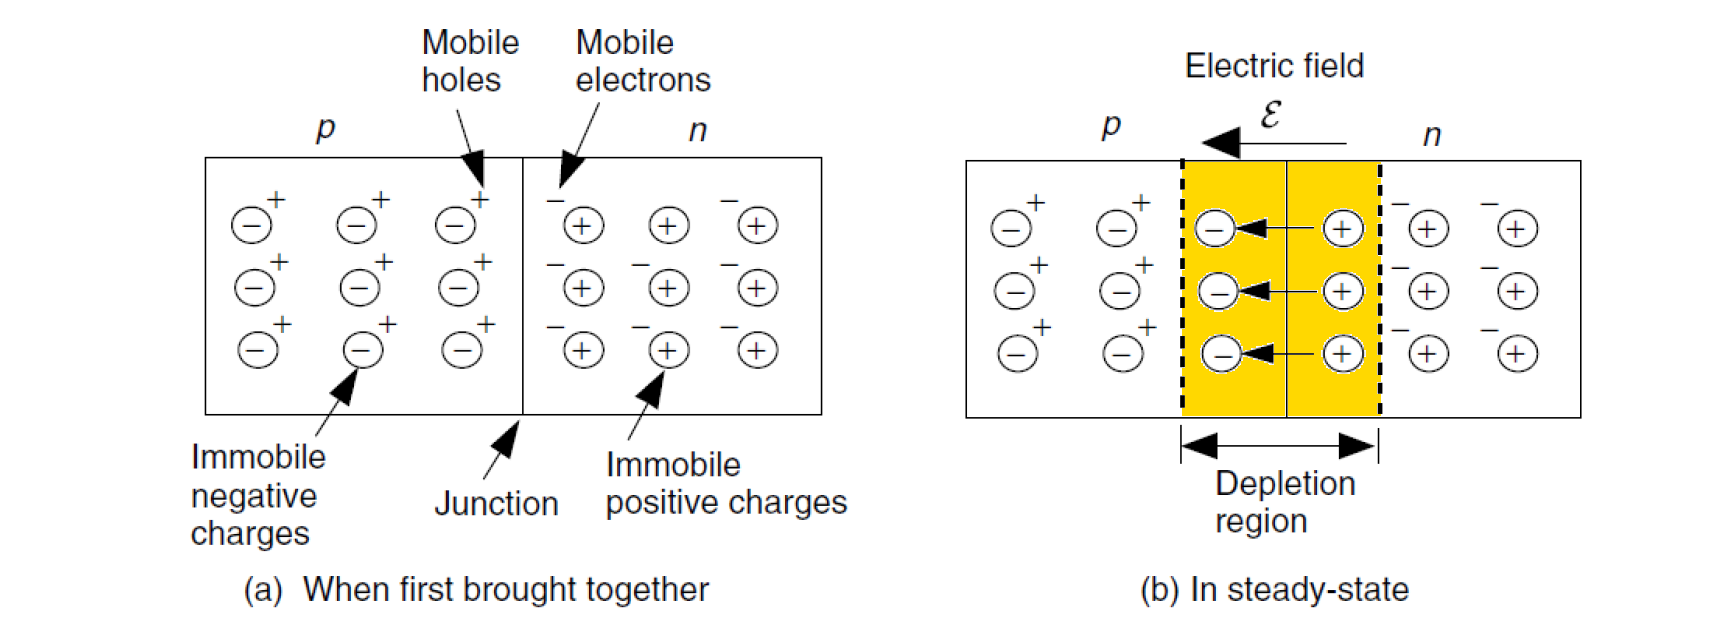
\includegraphics[width=\textwidth,height=\textheight,keepaspectratio]{immagini/1.png}
\caption{Regione di svuotamento}
\end{subfigure}
\begin{subfigure}[t]{0.3\textwidth}
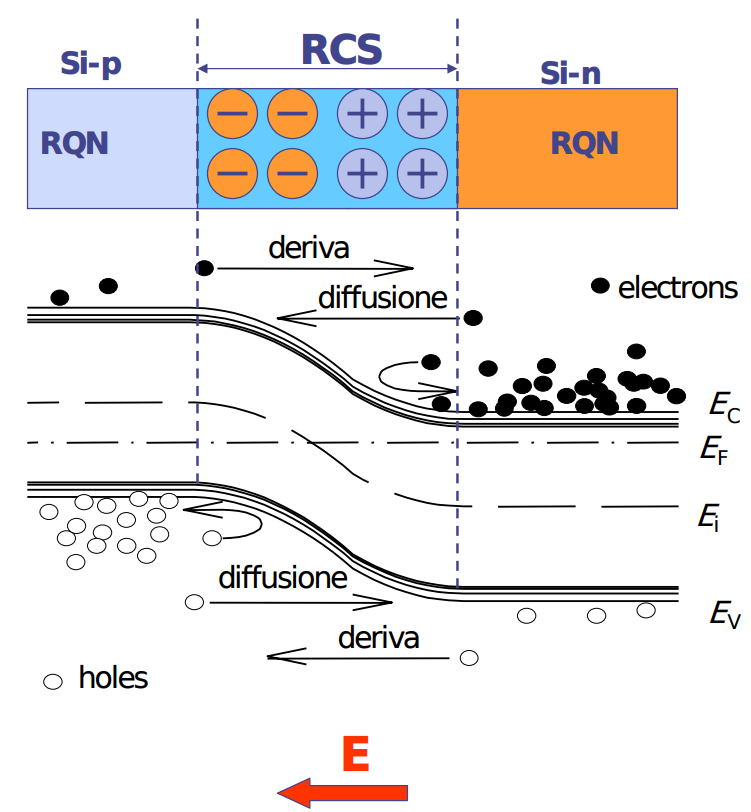
\includegraphics[width=\textwidth,height=\textheight,keepaspectratio]{immagini/pn_equilibrio.png}
\caption{Giunzione pn all'equilibrio}
\end{subfigure}
\end{figure}

In genere la regione di svuotamento non è simmetrica: la seguente
equazione regola la larghezza della regione: \[
x_p N_A = x_N N_D
\] dove \(x_p\) e \(x_n\) sono rispettivamente le \textbf{larghezze}
della regione di svuotamento entro il semiconduttore drogato p e drogato
n.

\begin{figure}[H]
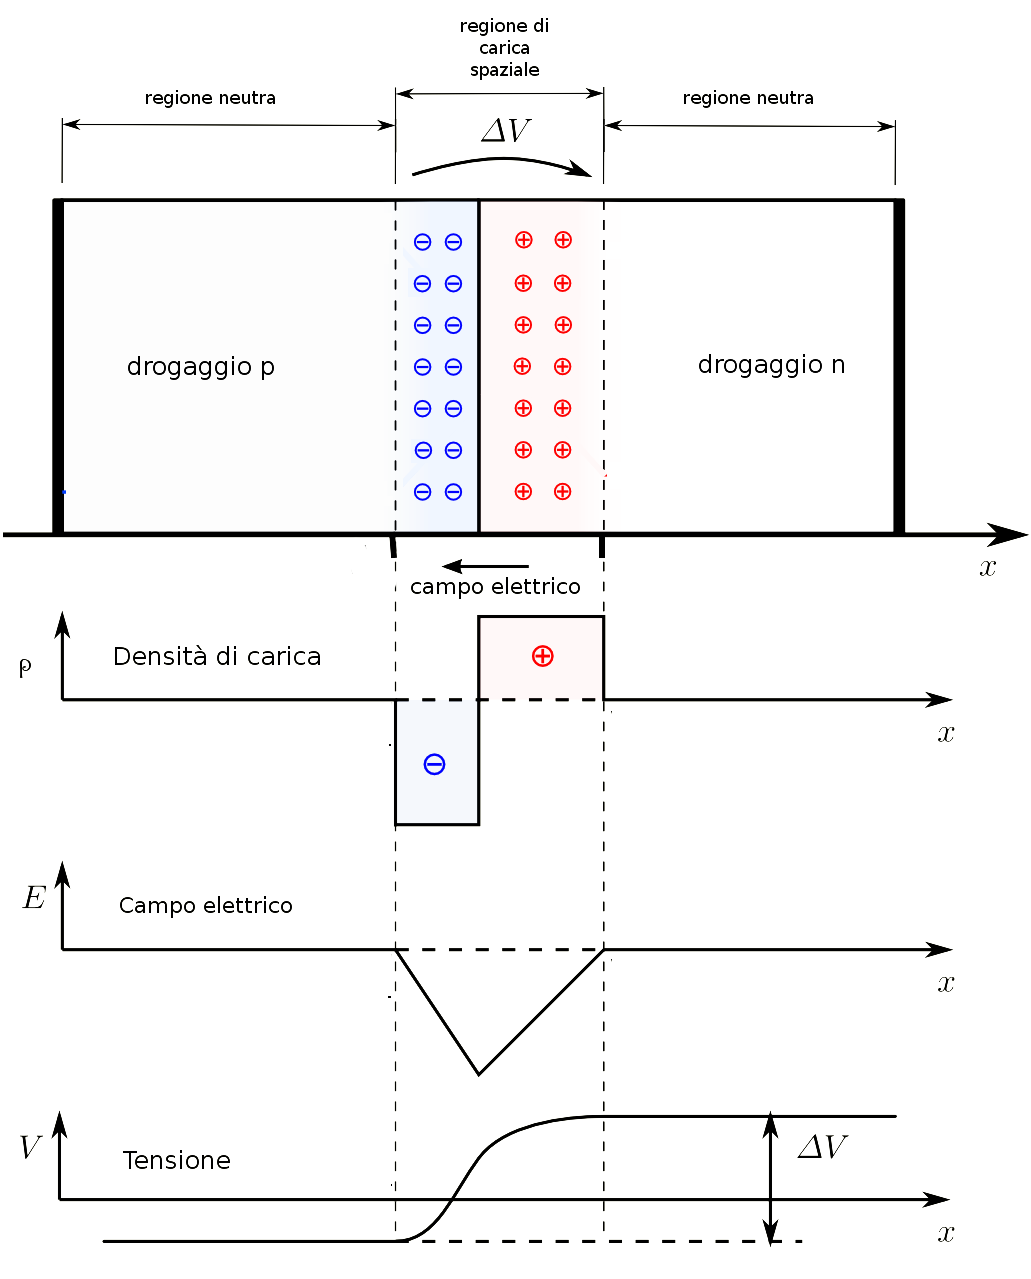
\includegraphics[height=0.6\textwidth, width=!]{immagini/2.png}
\centering
\caption{Grafici relativi al potenziale, al campo elettrico e alla carica nella giunzione pn}
\label{fig:1.3}
\end{figure}

Come si vede nella @fig:1.3 :

\begin{itemize}
\tightlist
\item
  \(N_A > N_D \to\) più è drogata la regione più la regione di
  svuotamento è piccola.
\end{itemize}

\subsection{Diodo}\label{diodo}

Il simbolo circuitale della giunzione p-n, detta
\textbf{diodo}\footnote{Il diodo ideale è un dispositivo che lascia
  passare corrente solo in un senso, con resistenza nulla, e non lascia
  passare corrente nell'altro senso. Il diodo a giunzione approssima
  molto bene un diodo ideale, ed è l'elemento circuitale non lineare più
  importante.} è

\begin{figure}[h]
\begin{centering}
\begin{circuitikz}
  \draw (0,0) node[left]{A} to[diode,color=red] (2,0) node[right]{K};
\end{circuitikz}
\caption{Diodo}
\end{centering}
\end{figure}

dove a sinistra abbiamo un \textbf{anodo} A (dal greco \emph{salita}), e
a destra un \textbf{catodo} K (dal greco \emph{discesa}).

Sia la zone p che la zona n sono munite di un contatto elettrico (detto
\textbf{reoforo}), in modo tale che sia possibile applicarvi una
tensione. È da notare come la zona n in contatto col suo reoforo deve
essere molto drogata \colorbox{yellow}{(approfondire)}.

\subsubsection{Polarizzazione}\label{polarizzazione}

L'applicazione di un potenziale sul diodo viene detta
\textbf{polarizzazione}, e si distingue la:

\begin{itemize}
\tightlist
\item
  Polarizzazione \textbf{diretta} (forward bias): applico un potenziale
  positivo sull'anodo A (lato p) e negativo sul catodo K (lato n). La
  differenza di potenziale applicata ha la polarità \emph{concorde} con
  la barriera di potenziale.

  \begin{itemize}
  \tightlist
  \item
    L'aumento della tensione determina una riduzione della barriera di
    potenziale, e di conseguenza della larghezza della regione di
    svuotamento. In questo modo aumenta il numero di elettroni e di
    lacune capaci di attraversare la giunzione tramite la diffusione.
  \item
    La corrente di diffusione, rispetto a quella di deriva, aumenta
    rapidamente di svariati ordini di grandezza.

    \begin{figure}[h]
    \begin{centering}
    \begin{circuitikz}
    \draw (0,0) node[left]{+} to[diode,color=blue] (2,0) node[right]{-};
    \end{circuitikz}
    \caption{Diodo polarizzato direttamente}
    \end{centering}
    \end{figure}
  \end{itemize}
\item
  Polarizzazione \textbf{indiretta} (reverse bias): applico un
  potenziale negativo sull'anodo e positivo sul catodo. In questo caso
  la polarità della tensione applicata è discorde rispetto a quella
  della barriera di potenziale.

  \begin{itemize}
  \tightlist
  \item
    La regione di svuotamento si allarga, e la tensione di
    polarizzazione richiama le lacune verso il terminale negativo e gli
    elettroni verso il terminale positivo. Quindi l'ampiezza della
    barriera di potenziale aumenta.
  \item
    La corrente di diffusione diminuisce fino ad annullarsi, mentre
    quella di deriva rimane (anche se è molto piccola e varia con la
    temperatura).
  \end{itemize}
\end{itemize}

\begin{figure}[h]
\begin{centering}
\begin{circuitikz}
  \draw (0,0) node[left]{-} to[diode,color=orange] (2,0) node[right]{+};
\end{circuitikz}
\caption{Diodo polarizzato indirettamente}
\end{centering}
\end{figure}

\subsubsection{Diodi Speciali}\label{diodi-speciali}

\begin{center}
\begin{circuitikz}
  \draw (0,0) node[left]{+} to[diode, l_=Diodo normale] (2,0) node[right]{-};
  \draw (4,0) node[left]{-} to[diode, l_=Fotodiodo] node[right]{+} (6,0);
\end{circuitikz}
\end{center}

\appendix

\chapter{Esercizi}\label{esercizi}

\section{Esercizi capitolo 1}\label{esercizi-capitolo-1}

\chapter{Varie}\label{varie}

\section{Semiconduttori e bande}\label{semiconduttori-e-bande}

Gli elettroni in un solido allo stato fondamentale e a temperatura \(0\)
kelvin, in obbedienza alla loro natura fermionica e al principio di
Pauli che preclude ai fermioni il fatto di potersi trovare in due nello
stesso stato, riempiono gli stati elettronici loro consentiti partendo
dal livello energetico più basso via via su, fino a che tutti gli
elettroni del solido hanno trovato un'accomodazione. Si distribuiscono
cioè rispettando la distribuzione di Fermi-Dirac calcolata a temperatura
0 kelvin. Nei metalli, il livello energetico più alto occupato si
definisce livello di Fermi.

\begin{figure}
\centering
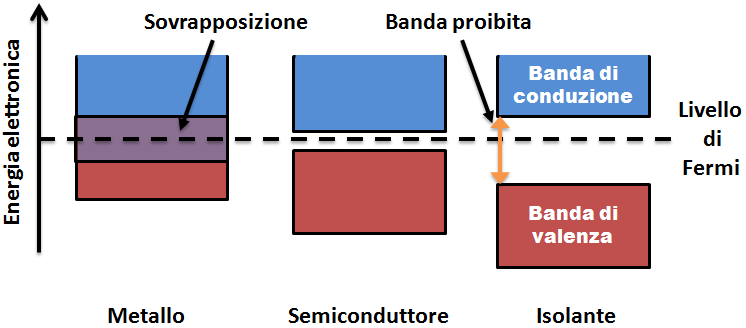
\includegraphics[width=0.5\linewidth,height=\textheight,keepaspectratio]{immagini/bande.png}
\caption{Schema semplificato della struttura elettronica a bande per
metalli, semiconduttori e isolanti.}
\end{figure}

A questo punto possono verificarsi diverse possibilità:

\begin{itemize}
\tightlist
\item
  Vi è una banda, o più di una fra le ultime riempite da elettroni, che
  è parzialmente riempita e restano degli stati vuoti. In tal caso si ha
  a che fare con un metallo, cioè un sistema in cui gli ultimi elettroni
  hanno la possibilità di spostarsi in livelli energetici molto vicini,
  infinitesimalmente più alti in energia, e dunque hanno la possibilità
  di una mobilità elevata che porta il sistema ad essere un buon
  conduttore di elettricità.
\item
  L'ultima banda è stata riempita completamente in modo tale che il
  prossimo stato elettronico consentito si trovi sulla banda successiva
  e fra questa banda e la banda completamente riempita c'è una banda
  proibita (\emph{band gap}) di energie. In tal caso il solido è un
  dielettrico.
\item
  Si parla infine di semiconduttore nel caso di un isolante in cui la
  banda proibita è talmente piccola che a temperatura ambiente c'è una
  certa probabilità che gli elettroni si trovino a saltare la banda
  proibita per agitazione termica, e dunque il sistema si trovi in una
  situazione prossima a quella di un metallo, con valori di
  conducibilità elettrica non nulli.
\end{itemize}

(N.B paragrafo proveniente da
\href{https://it.wikipedia.org/wiki/Struttura_elettronica_a_bande}{Wikipedia})

\backmatter
\end{document}
